
%(BEGIN_QUESTION)
% Copyright 2014, Tony R. Kuphaldt, released under the Creative Commons Attribution License (v 1.0)
% This means you may do almost anything with this work of mine, so long as you give me proper credit

Sketch the necessary wire connections for this bank of step-down transformers, so that the primary is in a ``Wye'' configuration and the secondary is in a ``Delta'' configuration.  Your sketched wires must connect the transformers to the primary and secondary busses as well as connect the transformers to each other.  There are no requirements for a particular amount of phase shift between primary and secondary phasor diagrams, nor do you need to worry about phase rotation:

$$\includegraphics[width=15.5cm]{i03316x01.eps}$$

\underbar{file i03316}
%(END_QUESTION)





%(BEGIN_ANSWER)

{\it Any} connection scheme is acceptable, so long as the specified configurations are there.  Phase rotation and phase shift from primary to secondary are irrelevant for the scope of this question:

$$\includegraphics[width=15.5cm]{i03316x02.eps}$$

%(END_ANSWER)





%(BEGIN_NOTES)

{\bf This question is intended for exams only and not worksheets!}.

%(END_NOTES)


